% !TeX root = main.tex

%\setkeys{Gin}{draft}

\onehalfspacing
\section{Lab Assignment Goals}
\justifying 

The goal of this lab was to study and compare the MOSFET-resistor biasing circuit and the beta multiplier circuit, specifically focusing on performance metrics such as power supply sensitivity. Biasing is essential in integrated circuits to establish proper operating points for transistors, ensuring consistent performance and linearity despite variations in temperature, power supply, or transistor parameters. The beta multiplier circuit is often preferred over a simple MOSFET-resistor configuration due to its ability to provide a more stable and predictable bias current, making it less sensitive to process and temperature variations. This stability is achieved through a feedback loop and multiple transistors that generate a reference current capable of adapting to changes, improving control and reliability in precision applications.  

To accomplish this, both circuits were simulated in LTSpice and built on a breadboard using the ALD1106/ALD1105 transistor array. Simulations and experimental measurements were conducted to analyze circuit behavior under different conditions, particularly variations in supply voltage. Data from both approaches were compared to evaluate the performance differences between the two biasing methods and to assess the advantages of the beta multiplier over the MOSFET-resistor configuration.

\begin{center}
\begin{figure}[ht]
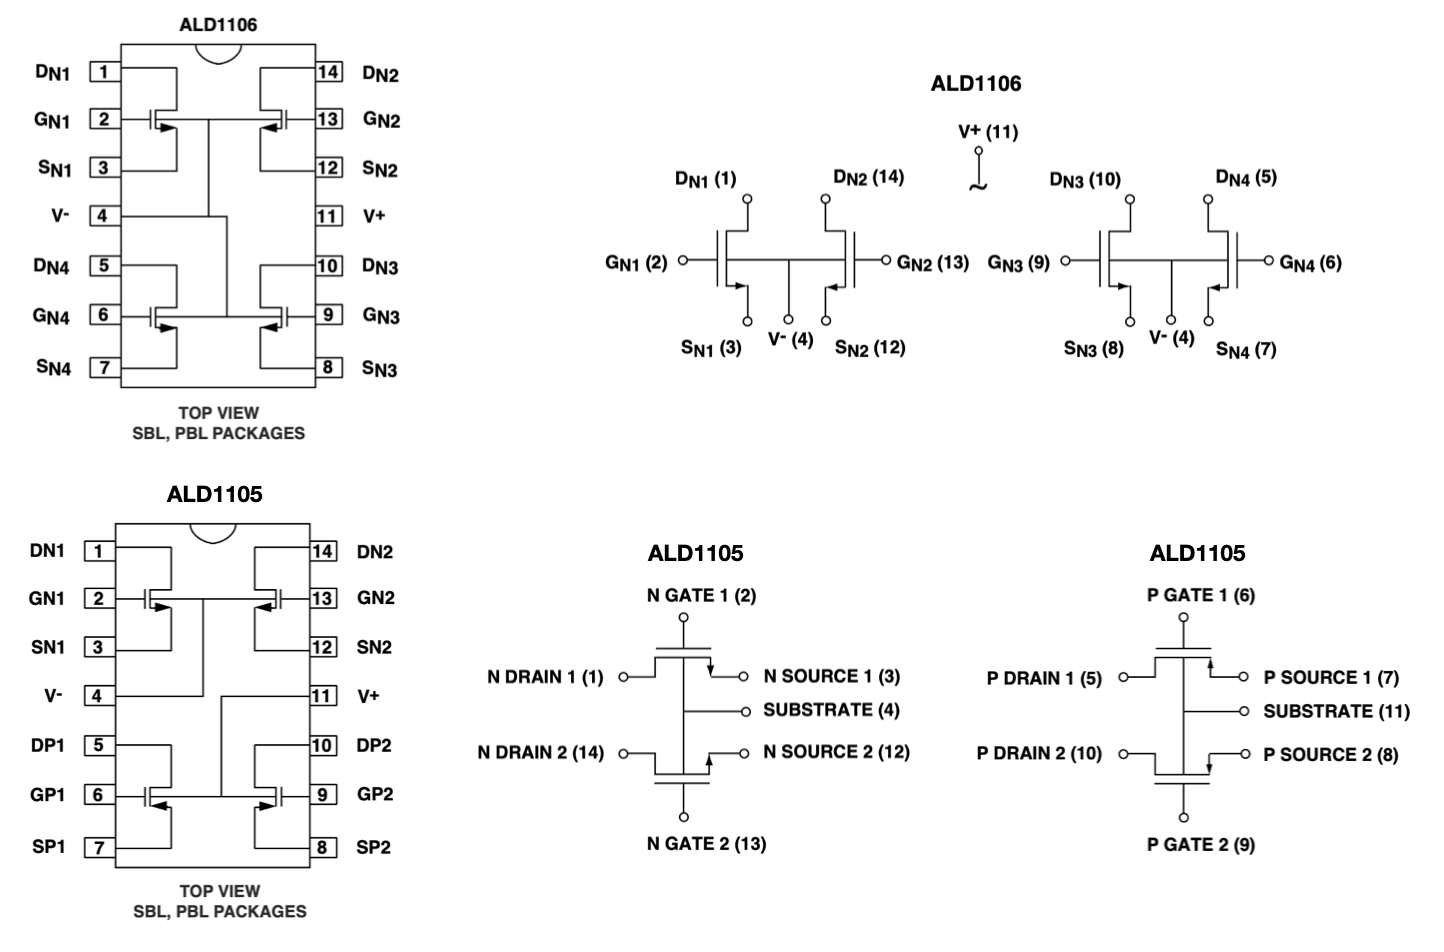
\includegraphics[scale=0.5\linewidth]{Chapter_2/Lab_02_Image_1.png}
\caption{The pinout and block diagram of the ALD1106 (top) and ALD1105 (bottom), \textbf{Note: $V^{-}$ is the body of the NMOS devices which is connected to lowest potential and $V^{+}$ is the body of the PMOS devices which is connected to the highest potential. }}
\label{fig:Ch2_fig1}
\end{figure}
\end{center}

\section{Experiment 1: The MOSFET-Resistor Characterization}

The objectives of this experiment involved characterizing a MOSFET-resistor circuit, as illustrated in the schematic below. The following tasks were performed:

\begin{itemize}
    
    \item The resistor was replaced with a 20k$\Omega$ potentiometer while setting $V_{DD} = 10$V. The resistance $R$ was determined at which $I_{D} = 500\mu$A.
    \item With the current set to $I_{D} = 500\mu$A, the DC operating point was identified.
    \item Finally, the supply voltage $V_{DD}$ was swept from 0 to 15V.
    
\end{itemize}

\begin{center}

\begin{circuitikz}[american]
\ctikzset{tripoles/mos style=arrows}

\draw

(0,0) node[nmos,scale=2] (Q1) {}
(Q1.center) node[right] {$Q_{1}$}
(Q1.S) node[ground] {} 
(Q1.D) to[R=$R$] ++(0,3) node[vcc] (vcc) {$+V_{DD}$}
(Q1.G) to[short] ++(-1,0) to[short] ++(0,1.5) to[short,-*] ++(2.96,0)

;   
\end{circuitikz}
\end{center}

\begin{center}
	\begin{figure}[ht]
	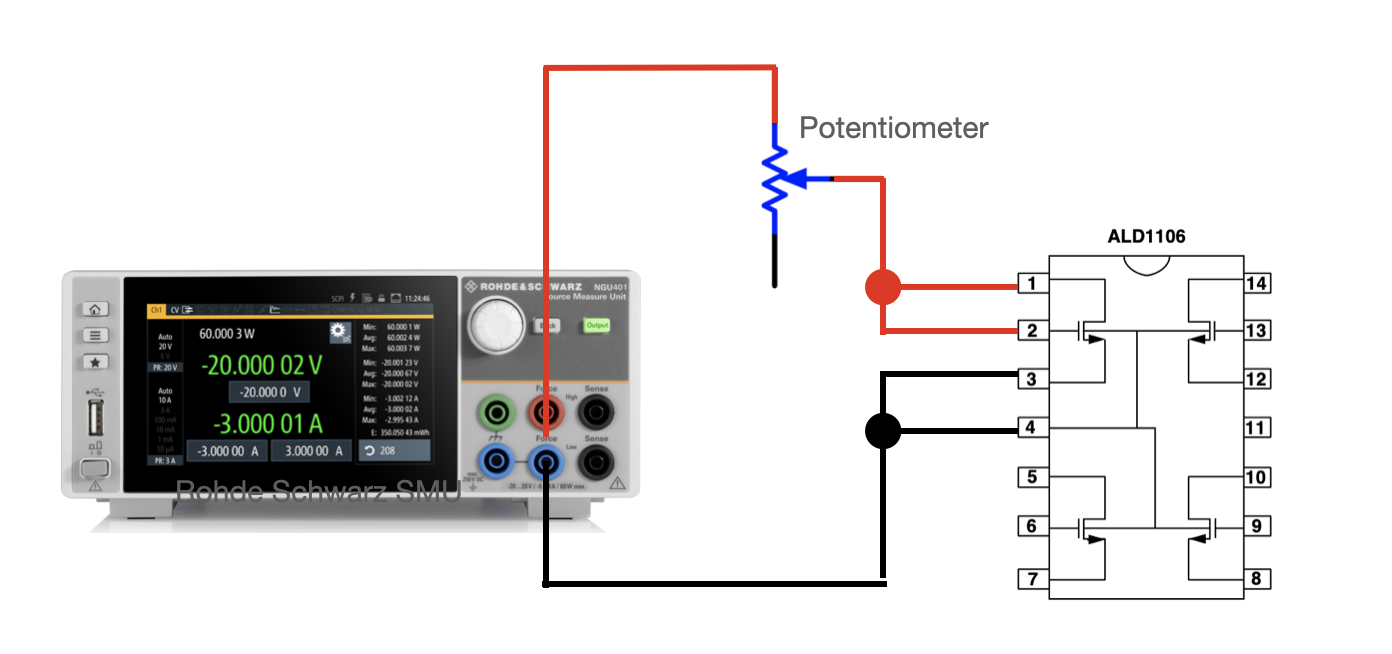
\includegraphics[scale=0.475\linewidth]{Chapter_2/Lab_02_Image_2.png}
	\caption{Wiring diagram of the MOSFET-resistor biasing circuit. The potentiometer had three terminals, with the top and bottom terminals used in combination with the middle terminal. }
	\label{Ch2_fig:2}
	\end{figure}
\end{center}

\newpage



%\newpage
\section{Experiment 2: The Beta Multiplier Characterization}

The objectives of this experiment involved characterizing a beta multiplier circuit, as illustrated in the schematic below. The following tasks were performed. Additionally, the width of $Q_{2}$ was four times that of $Q_{1}$, achieved by wiring four NMOS devices in parallel as available on the ALD1106:

\begin{itemize}

    \item The resistor was replaced with a 5k$\Omega$ potentiometer while setting $V_{DD} = 10$V. The resistance $R$ was determined at which $I_{D2} = 500\mu$A.
    \item With the current set to $I_{D2} = 500\mu$A, the DC operating point was identified.
    \item Finally, the supply voltage $V_{DD}$ was swept from 0 to 15V.
    \item Python Code used for this experiment can be found under the code listings~\cref{Ch2:List1}, ~\cref{Ch2:List2}, \& ~\cref{Ch2:List3}
    
\end{itemize}

\begin{center}

\begin{circuitikz}[american]
\ctikzset{tripoles/mos style=arrows}

\draw

(3,2) node[pmos,scale=1.5] (Q4) {}
(3,-2) node[nmos,scale=1.5] (Q2) {}
(-3,2) node[pmos,scale=1.5,xscale=-1] (Q3) {}
(-3,-2) node[nmos,scale=1.5,xscale=-1] (Q1) {}
(Q4.S) node[vcc] (vcc) {$+V_{DD}$}
(Q3.S) node[vcc] (vcc) {$+V_{DD}$}
(Q4.G) -- (Q3.G)
(Q1.G) -- (Q2.G)
(Q1.D) -- (Q3.D)
(Q2.D) -- (Q4.D)
(Q1.S) node[ground] {}
(Q2.S) to[R=$R$] ++(0,-2) node[ground] {}
(Q1.D) to[short,*-] ++(2,0) to[short,-*] ++(0,-1.15)
(Q4.D) to[short,*-] ++(-2,0) to[short,-*] ++(0,1.15)
(Q1.center) node[left] {$Q_{1}$}
(Q3.center) node[left] {$Q_{3}$}
(Q2.center) node[right] {$Q_{2}$}
(Q4.center) node[right] {$Q_{4}$}

;   
\end{circuitikz}

\begin{figure}[ht]
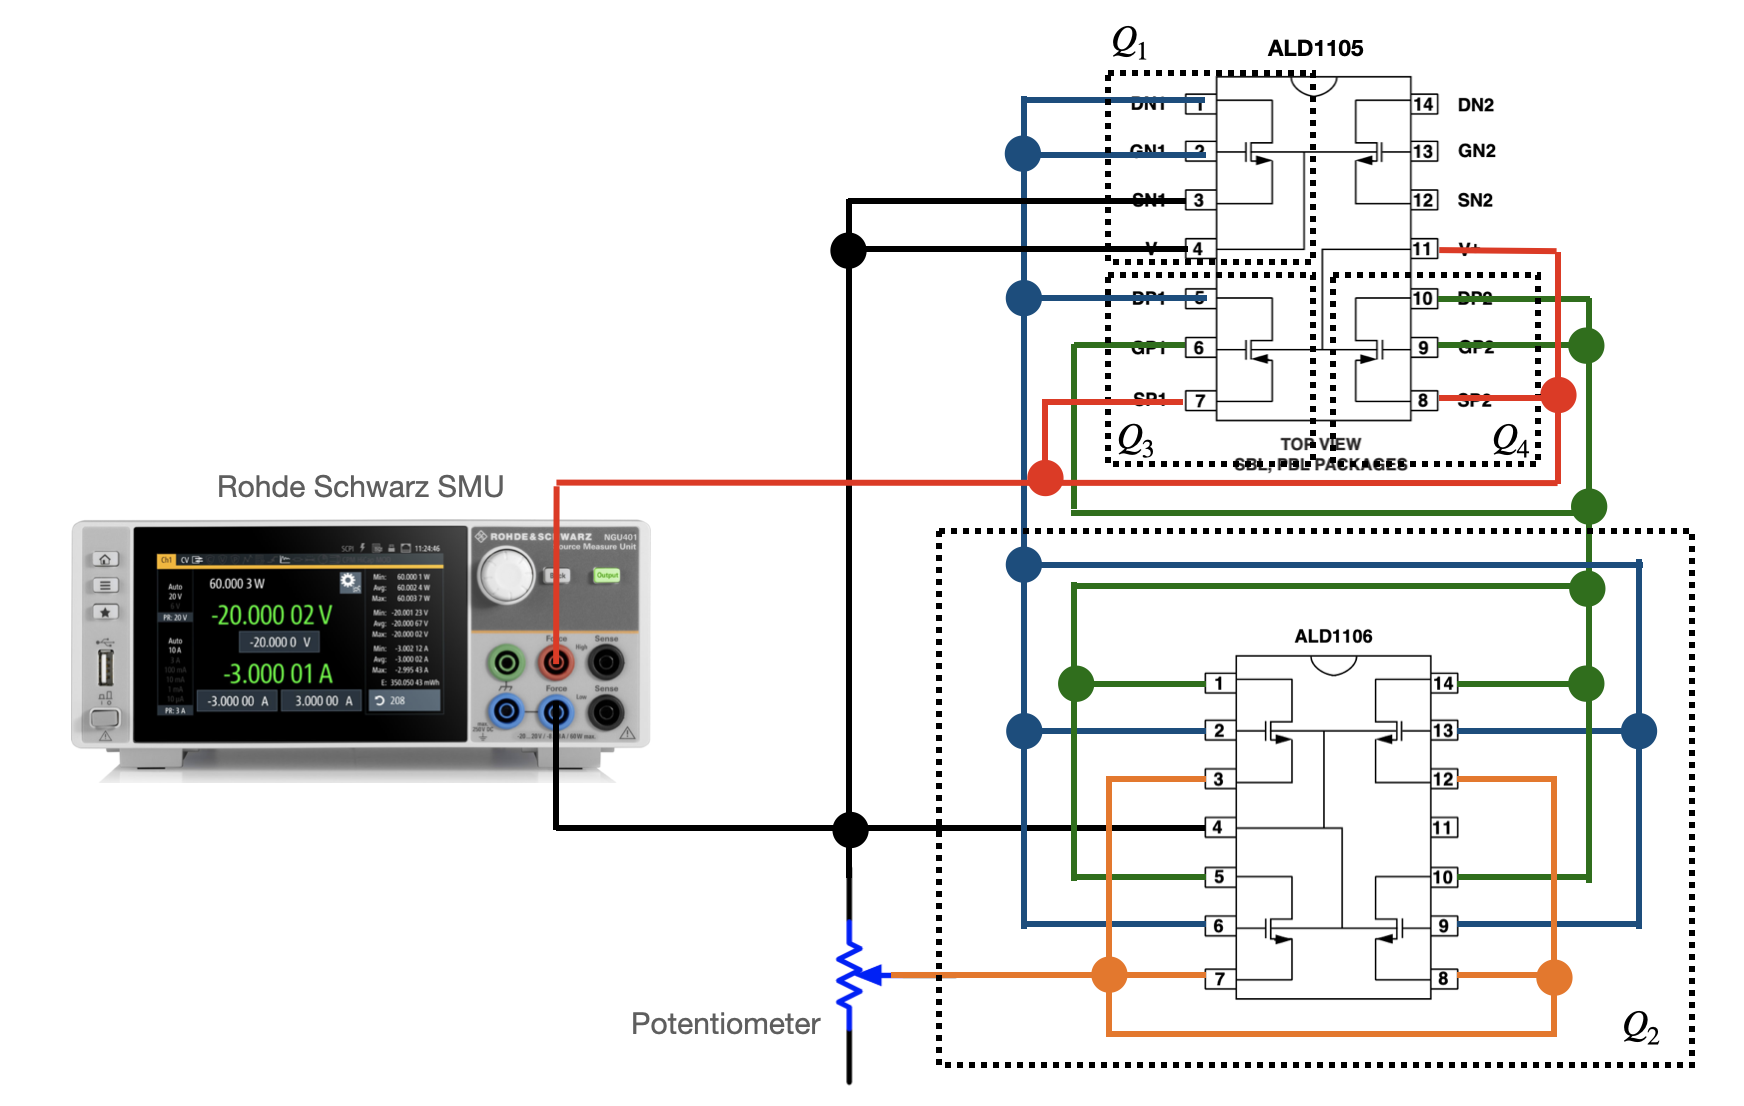
\includegraphics[scale=0.475\linewidth]{Chapter_2/Lab_02_Image_3.png}
\caption{Wiring diagram of the MOSFET-resistor biasing circuit. The potentiometer had three terminals, with the top and bottom terminals used in combination with the middle terminal. }
\label{Ch2_fig:2a}
\end{figure}

\end{center}

\newpage

\section{Post Lab Data Analysis}

The post-lab analysis involved the following tasks:

\begin{itemize}

    \item The circuits from Experiment 1 and Experiment 2 were simulated, following the same procedure of sweeping $R$ to determine the bias point at $I_{D} = I_{D2} = 500\mu$A. The DC operating point was then identified, followed by sweeping the power supply $V_{DD}$ from 0 to 15V.
    \item The tables for simulated and measured data were completed as specified.
    \item Both the simulated and measured power supply voltage sweeps were plotted on the same curve. The derivative of the simulated data was taken to determine the supply voltage sensitivity at the operating point $V_{DD} = 10$V.
    \item The results from Experiment 1 and Experiment 2 were compared to determine which circuit exhibited greater resistance to dynamic changes in the power supply.
    
\end{itemize}

\subsection{Experiment 1 - Results:}

\begin{center}
\begin{figure}[H]
	\centering
	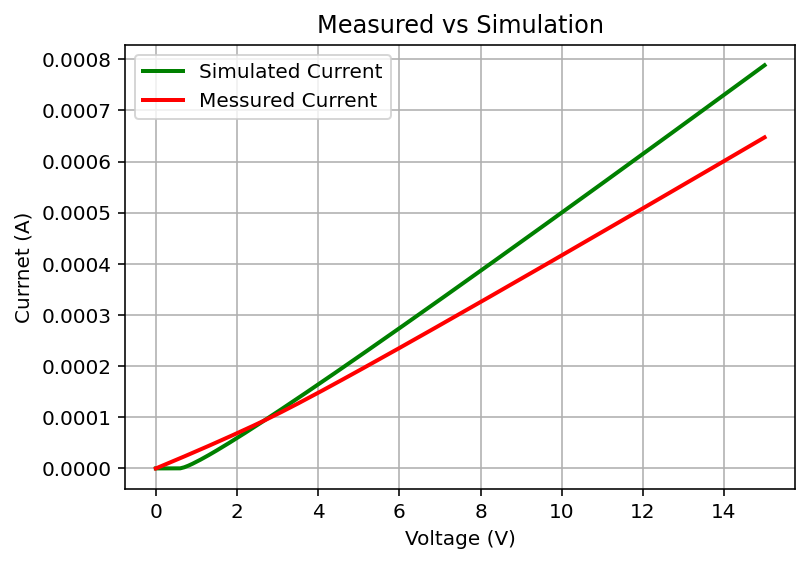
\includegraphics[width=0.65\linewidth]{Chapter_2/Lab_02_Exp_01_SIM_VS_MEAS_FINAL.png}
	\caption{Experiment 1: Simulated vs Measured Plot}
	\label{Ch2fig:1}
\end{figure}
\end{center}

\begin{center}
\begin{table}[H]
\begin{tabular}{| >{\centering\arraybackslash} m{3cm} | >{\centering\arraybackslash} m{3cm} | >{\centering\arraybackslash} m{3cm} | >{\centering\arraybackslash} m{2cm} |}
	\hline
	Quantity & Simulated & Measured & Units \\
	\hline
	$R$ & 16.200 & 16.003 & k$\Omega$ \\
	\hline
	$V_{GS1}$ & 1.91 & 1.940 & V \\
	\hline
	$V_{DS1}$ & 1.91 & 1.940 & V \\
	\hline
	$V_{OV1}$ & 1.337 & 1.341 & V \\
	\hline
	$I_{D1}$ & 499.999 & 504.477 & $\mu$A \\
	\hline
\end{tabular}
\caption{Experiment 1 Data Summary}
\end{table}
\end{center}

\newpage

\subsection{Experiment 2 - Simulated Results:}
The post-lab analysis involved comparing two circuit configurations, with the data clearly demonstrating that the circuit from Experiment 2 exhibits superior resistance to sudden changes in the power supply voltage. This enhanced stability can be attributed to the beta mirror configuration, which employs a cascade of current mirrors to maintain consistent current flow. The multiple transistor stages in the beta mirror create a high-impedance path that effectively isolates the bias current from power supply fluctuations. Additionally, the negative feedback inherent in the mirror configuration helps compensate for any variations in supply voltage by adjusting the gate-source voltages of the transistors to maintain constant current.
\vspace{0.25cm}

\begin{center}
	\begin{figure}
		\centering
		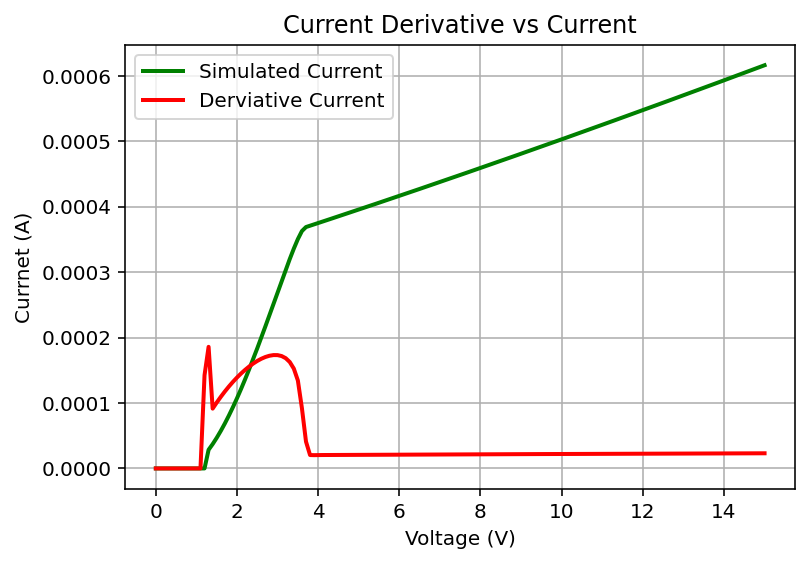
\includegraphics[scale=0.4]{Chapter_2/Lab_02_Exp_02_SIM_ID_vs_Derivative_Plot_FINAL.png}
		\caption{Experiment 2: Simulated $I_D$ vs $\frac{d}{dt}(I_D)$ Plot}
		\label{Ch2fig:2}
	\end{figure}
\end{center}

\begin{center}
\begin{table}[H]
\scriptsize
%	\renewcommand{\arraystretch}{1.4}
\setlength{\tabcolsep}{4pt} % default is 6pt
\begin{tabular}{| >{\centering\arraybackslash} m{3cm} | >{\centering\arraybackslash} m{3cm} | >{\centering\arraybackslash} m{3cm} | >{\centering\arraybackslash} m{2cm} |}
\hline
Quantity & Simulated & Measured & Units \\
\hline
$R$ & 1.254 & 1.0361 & k$\Omega$ \\
\hline
$V_{GS1}$ & 1.980 & 1.985 & V \\
\hline
$V_{DS1}$ & 1.980 & 1.985 & V \\
\hline
$V_{OV1}$ & 1.407 & 1.424 & V \\
\hline
$I_{D1}$ & 552.000 & 506.814 & $\mu$A \\
\hline
$V_{GS2}$ & 1.350 & 1.496 & V \\
\hline
$V_{DS2}$ & 6.420 & 6.646 & V \\
\hline
$V_{OV2}$ & 0.644 & 0.935 & V \\
\hline
$I_{D2}$ & 500.000 & 506.814 & $\mu$A \\
\hline
$V_{SG3}$ & 2.960 & 2.861 & V \\
\hline
$V_{SD3}$ & 8.020 & 8.006 & V \\
\hline
$|V_{OV3}|$ & 2.313 & 2.399 & V \\
\hline
$I_{D3}$ & 552.000 & 506.814 & $\mu$A \\
\hline
$V_{SG4}$ & 2.960 & 2.862 & V \\
\hline
$|V_{OV4}|$ & 2.313 & 2.301 & V \\
\hline
$I_{D4}$ & 500.000 & 506.814 & $\mu$A \\
\hline
\end{tabular}
\caption{Experiment 2 Data Summary}
\end{table}
\end{center}


\subsection{Experiment 2 - Simulated vs Measured Results:}

\begin{center}
	\begin{figure}[ht]
		\centering
		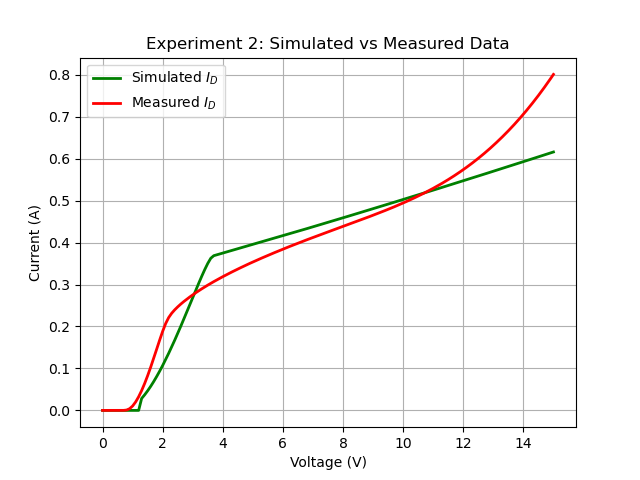
\includegraphics[scale=0.4]{Chapter_2/Lab_02_Exp_2_Sim_vs_Meas_Plot_FINAL.png} 
		\caption{Experiment 2: Simulated vs Measured Plots}
		\label{Ch2fig:3}
	\end{figure}
\end{center}

\section{Code Listings}

The Python implementations for the biasing analysis can be found in the Appendix: Plot Measured vs Simulated Data (\cref{lst:Ch2:List1}), Extract OP Values from LTSpice (\cref{lst:Ch2:List2}), Plot Measured vs Simulated Current (\cref{lst:Ch2:List3}), Calculate MOSFET Parameters (\cref{lst:Ch2:List4}), and Simulated vs Measured Data Plot (\cref{lst:Ch2List5}).

\section{Conclusion}
\justifying
This lab effectively demonstrated the differences in performance and robustness between a basic MOSFET-resistor biasing circuit and a beta multiplier biasing configuration. Through both simulation and physical prototyping, it was observed that while the MOSFET-resistor circuit can achieve the desired operating point with manual tuning, it suffers from significant sensitivity to changes in supply voltage. In contrast, the beta multiplier circuit consistently maintained a stable bias current across varying supply voltages, showcasing superior power supply rejection characteristics.

The enhanced stability of the beta multiplier can be attributed to its negative feedback mechanism and the use of matched transistor pairs, which allow the circuit to self-correct and adapt to fluctuations in external conditions. This makes it a preferred choice in precision analog and mixed-signal applications where stability and predictability are crucial.

Simulation results closely matched experimental data for both circuits, validating the modeling approach in LTSpice. Additionally, the derivative analysis confirmed that the beta multiplier exhibited a flatter response in current with respect to changes in $V_{DD}$​, quantitatively proving its reduced supply voltage sensitivity.

Overall, results highlight the importance of choosing appropriate biasing strategies in analog design and illustrated the trade-off between simplicity and performance in circuit design.


% \end{document}
